\documentclass[12pt]{amsart}

\addtolength{\hoffset}{-2.25cm}
\addtolength{\textwidth}{4.5cm}
\addtolength{\voffset}{-2.5cm}
\addtolength{\textheight}{5cm}
\setlength{\parskip}{0pt}
\setlength{\parindent}{15pt}

\usepackage{amsthm}
\usepackage{amsmath}
\usepackage{amssymb}
\usepackage{ctex}

\usepackage[colorlinks = true, linkcolor = black, citecolor = black, final]{hyperref}

\usepackage{graphicx}
\usepackage{multicol}
\usepackage{marvosym}
\usepackage{wasysym}
\usepackage{tikz}
\usepackage{listings}
\usepackage{xcolor}
\usepackage{subcaption}


\definecolor{codegreen}{rgb}{0,0.6,0}
\definecolor{codegray}{rgb}{0.5,0.5,0.5}
\definecolor{codepurple}{rgb}{0.58,0,0.82}
\definecolor{backcolour}{rgb}{0.95,0.95,0.92}

\lstdefinestyle{mystyle}{
    backgroundcolor=\color{backcolour},   
    commentstyle=\color{codegreen},
    keywordstyle=\color{magenta},
    numberstyle=\tiny\color{codegray},
    stringstyle=\color{codepurple},
    basicstyle=\ttfamily\footnotesize,
    breakatwhitespace=false,         
    breaklines=true,                 
    captionpos=b,                    
    keepspaces=true,                 
    numbers=left,                    
    numbersep=5pt,                  
    showspaces=false,                
    showstringspaces=false,
    showtabs=false,                  
    tabsize=2
}

\lstset{style=mystyle}

\usepackage{color}
\definecolor{gray}{rgb}{0.4,0.4,0.4}
\definecolor{darkblue}{rgb}{0.0,0.0,0.6}
\definecolor{cyan}{rgb}{0.0,0.6,0.6}

\lstset{
  basicstyle=\ttfamily,
  columns=fullflexible,
  showstringspaces=false,
  commentstyle=\color{gray}\upshape
}

\lstdefinelanguage{XML}
{
  numbers=left,
  morestring=[b]",
  morestring=[s]{>}{<},
  morecomment=[s]{<?}{?>},
  stringstyle=\color{black},
  identifierstyle=\color{darkblue},
  keywordstyle=\color{cyan},
  morekeywords={xml,version,type,ELEMENT,PCDATA}% list your attributes here
}
\lstdefinelanguage{DTD}
{
  numbers=left,
  morestring=[b]",
  morestring=[s]{>}{<},
  morecomment=[s]{<?}{?>},
  stringstyle=\color{black},
  identifierstyle=\color{darkblue},
  keywordstyle=\color{cyan},
  morekeywords={xmlns,version,type,ELEMENT,PCDATA}% list your attributes here
}

\usetikzlibrary{patterns}

\newcommand{\ds}{\displaystyle}

\setlength{\parindent}{2em}

\pagestyle{empty}

\begin{document}

\thispagestyle{empty}

\noindent{\scshape EC 5001} \hfill {\scshape \large Individual assignment (XML)} \hfill HUANG Kunlun \hfill {\scshape P1}
 
\smallskip

\hrule

\bigskip

In this assignment, I design XML format files to represent
the receipt of wellcome supermarket (惠康超市)  (Figure \ref{fig:receipt1} \& Figure \ref{fig:receipt2} ).

\bigskip

Firstly, I design DTD format files (Listing \ref{lst:dtdfile}) to represent the receipts.
The DTD outlines the structure and constraints for an XML document representing a wellcomereceipt. The primary element, "wellcomereceipt," serves as the root and encompasses various essential components of a transaction receipt.

The essential components and their relationships within the receipt include:
\begin{itemize}
    \item Identification details such as branchName and branchPhoneNumber.
    \item Details of purchased Items which may include Item elements specifying the itemName, itemQuantity, itemPrice, and an optional applyDiscountType.
    \item Discounts applied, represented by the Discounts element containing one or more Discount elements, each specifying discountName, applyDiscountType, and discountPrice.
    \item Amount information presented through the Amount element, specifying totalAmount, totalDiscount, payAmount, and notCount.
    \item Payment-related details within the Payment element, encompassing paymentMethod, refNumber, terminalNumber, branchNumber, serialNumber, authCode, checkNumber, payAmount, and dealAmount.
    \item Temporal information captured by the transTime element.
    \item A unique barcode identifier, given by the barcodeNumer element.
    \item Optionally, additional offer information within the offerInfo element.
    \item A textual statement or warranty information presented in the statement element.
\end{itemize}

In essence, this DTD provides a comprehensive blueprint for structuring XML documents representing well-received transaction receipts, ensuring consistency and conformity to the specified format.

\bigskip

Then I tranfer two real receipt to the XML files  (Listing \ref{lst:xmlfile1} \& Listing \ref{lst:xmlfile2})  accouding to the DTD.

\bigskip

Finally, I design a simple HTML to display the XML file (Figure \ref{fig:html1} \& Figure \ref{fig:html2} ).



\bigskip

\bigskip

\bigskip

\bigskip

\bigskip

\bigskip

\bigskip

\bigskip

\bigskip

\bigskip

\bigskip

\hrule

\smallskip

Project Source Code: https://github.com/hiplon/CityUEC5001Assignment

\newpage

\noindent{\scshape EC 5001} \hfill {\scshape \large Individual assignment (XML)} \hfill HUANG Kunlun \hfill {\scshape P2}
 
 
\smallskip

\hrule

\bigskip

\noindent{\bf The wellcomereceipt DTD Files:}  

\smallskip

\begin{lstlisting}[caption={DTD file},label={lst:dtdfile},
    language=DTD,breaklines=true]
<!ELEMENT wellcomereceipt (branchName,branchPhoneNumber,Items,Discount?,Amount,Payment,transTime,Server,barcodeNumer,offerInfo?,statement)>
<!ELEMENT branchName (#PCDATA)>
<!ELEMENT branchPhoneNumber (#PCDATA)>
<!ELEMENT Items (Item+)>
<!ELEMENT Item (itemName,itemQuantity,itemPrice,applyDiscountType?)>
<!ELEMENT Discounts (Discount+)>
<!ELEMENT Discount (discountName,applyDiscountType,discountPrice)>
<!ELEMENT Amount (totalAmount,totalDiscount,payAmount,notCount)>
<!ELEMENT totalAmount (#PCDATA)>
<!ELEMENT totalDiscount (#PCDATA)>
<!ELEMENT payAmount (#PCDATA)>
<!ELEMENT notCount (#PCDATA)>
<!ELEMENT Payment (paymentMethod,refNumber,terminalNumber,branchNumber,serialNumber,authCode,checkNumber,payAmount,dealAmount)>
<!ELEMENT paymentMethod (#PCDATA)>
<!ELEMENT refNumber (#PCDATA)>
<!ELEMENT terminalNumber (#PCDATA)>
<!ELEMENT serialNumber (#PCDATA)>
<!ELEMENT authCode (#PCDATA)>
<!ELEMENT checkNumber (#PCDATA)>
<!ELEMENT displayAmount (#PCDATA)>
<!ELEMENT dealAmount (#PCDATA)>
<!ELEMENT transTime (#PCDATA)>
<!ELEMENT Server (#PCDATA)> 
<!ELEMENT barcodeNumer (#PCDATA)> 
<!ELEMENT offerInfo (#PCDATA)> 
<!ELEMENT statement (#PCDATA)> 
\end{lstlisting}

\newpage

\noindent{\scshape EC 5001} \hfill {\scshape \large Individual assignment (XML)} \hfill HUANG Kunlun \hfill {\scshape P3}
 
\smallskip

\hrule

\bigskip

\noindent{\bf XML receipt files 1:}  

\begin{lstlisting}[caption={XML file 1},label={lst:xmlfile1},
    language=XML,breaklines=true]
<?xml version="1.0"?>
<!DOCTYPE wellcomereceipt SYSTEM "wellcomereceipt.dtd">
<wellcomereceipt>
  <branchName>港湾豪庭</branchName>
  <branchPhoneNumber>31443783</branchPhoneNumber>
  <Items>
    <Item>
        <itemName>优惠速销</itemName>
        <itemQuantity>1</itemQuantity>
        <itemPrice>12</itemPrice>
    </Item>
    <Item>
        <itemName>公仔蒲烧鳗鱼味炒面王</itemName>
        <itemQuantity>1</itemQuantity>
        <itemPrice>7</itemPrice>
    </Item>
    <Item>
        <itemName>奇伟果</itemName>
        <itemQuantity>1</itemQuantity>
        <itemPrice>3.3</itemPrice>
    </Item>
    <Item>
        <itemName>百福鲜低糖豆浆236ML</itemName>
        <itemQuantity>1</itemQuantity>
        <itemPrice>5.5</itemPrice>
        <applyDiscountType>1</applyDiscountType>
    </Item>
    <Item>
        <itemName>百福无添加糖鲜豆浆236ML</itemName>
        <itemQuantity>2</itemQuantity>
        <itemPrice>5.5</itemPrice>
        <applyDiscountType>1</applyDiscountType>
    </Item>
  </Items>
  <Discounts>
    <Discount>
        <discountName>$12.5/3</discountName>
        <applyDiscountType>1</applyDiscountType>
        <discountPrice>-4</discountPrice>
    </Discount>
  </Discounts>
  <Amount>
    <totalAmount>38.8</totalAmount>
    <totalDiscount>-4</totalDiscount>
    <displayAmount>34.8</displayAmount>
    <notCount>0</notCount>
  </Amount>
  <Payment>
    <paymentMethod>WeChatPay</paymentMethod>
    <refNumber>231016220159</refNumber>
    <terminalNumber>21351005</terminalNumber>
    <branchNumber>852111154110001</branchNumber>
    <serialNumber>030974</serialNumber>
    <authCode>C09595</authCode>
    <checkNumber>42000020004202310167601534940</checkNumber>
    <payAmount>34.8</payAmount>
    <dealAmount>32.56</dealAmount>
  </Payment>
  <transTime>16102023/22:01</transTime>
  <Server>3512/005/4884/Sze Kuen</Server>
  <barcodeNumer>1610230002030054884</barcodeNumer>
  <offerInfo>You can join our XXXX activity for XXXXX.</offerInfo>
  <statement>some warrenty information and statements</statement>
</wellcomereceipt> 

\end{lstlisting}

\newpage
\noindent{\scshape EC 5001} \hfill {\scshape \large Individual assignment (XML)} \hfill HUANG Kunlun \hfill {\scshape P5}
 
\smallskip

\hrule

\bigskip

\noindent{\bf XML receipt files 2:}  

\begin{lstlisting}[caption={XML file 2},label={lst:xmlfile2},
    language=XML,breaklines=true]
<?xml version="1.0"?>
<!DOCTYPE wellcomereceipt SYSTEM "wellcomereceipt.dtd">
<wellcomereceipt>
  <branchName>港湾豪庭</branchName>
  <branchPhoneNumber>31443783</branchPhoneNumber>
  <Items>
    <Item>
        <itemName>壹品无添加糖豆浆500ML</itemName>
        <itemQuantity>1</itemQuantity>
        <itemPrice>8.5</itemPrice>
    </Item>
    <Item>
        <itemName>雪之恋抹茶红豆棉花大福</itemName>
        <itemQuantity>1</itemQuantity>
        <itemPrice>13</itemPrice>
    </Item>
    <Item>
        <itemName>巨浪大切香辣味薯片150GM</itemName>
        <itemQuantity>1</itemQuantity>
        <itemPrice>22</itemPrice>
        <applyDiscountType>2</applyDiscountType>
    </Item>
    <Item>
        <itemName>巨浪大切番茄味薯片150GM</itemName>
        <itemQuantity>1</itemQuantity>
        <itemPrice>22</itemPrice>
        <applyDiscountType>2</applyDiscountType>
    </Item>
  </Items>
  <Discounts>
    <Discount>
        <discountName>$24/2</discountName>
        <applyDiscountType>2</applyDiscountType>
        <discountPrice>-20</discountPrice>
    </Discount>
  </Discounts>
  <Amount>
    <totalAmount>65.5</totalAmount>
    <totalDiscount>-20</totalDiscount>
    <displayAmount>45.5</displayAmount>
    <notCount>0</notCount>
  </Amount>
  <Payment>
    <paymentMethod>WeChatPay</paymentMethod>
    <refNumber>231114220711</refNumber>
    <terminalNumber>21351061</terminalNumber>
    <branchNumber>852111154110001</branchNumber>
    <serialNumber>020438</serialNumber>
    <authCode>C02967</authCode>
    <checkNumber>4200001988202311141956032624</checkNumber>
    <payAmount>45.5</payAmount>
    <dealAmount>42.44</dealAmount>
  </Payment>
  <transTime>14112023/22:05</transTime>
  <Server>3512/061/7006/21351261</Server>
  <barcodeNumer>1411230002030617006</barcodeNumer>
  <statement>some warrenty information and statements</statement>
</wellcomereceipt> 

\end{lstlisting}

\newpage


\noindent\centering{\bf Figure: Real-World receipts from Wellcome}\label{fig:receipt}


\bigskip

\begin{figure}
  \centering
  \subcaptionbox{Wellcome Receipt 1\label{fig:receipt1}}
  {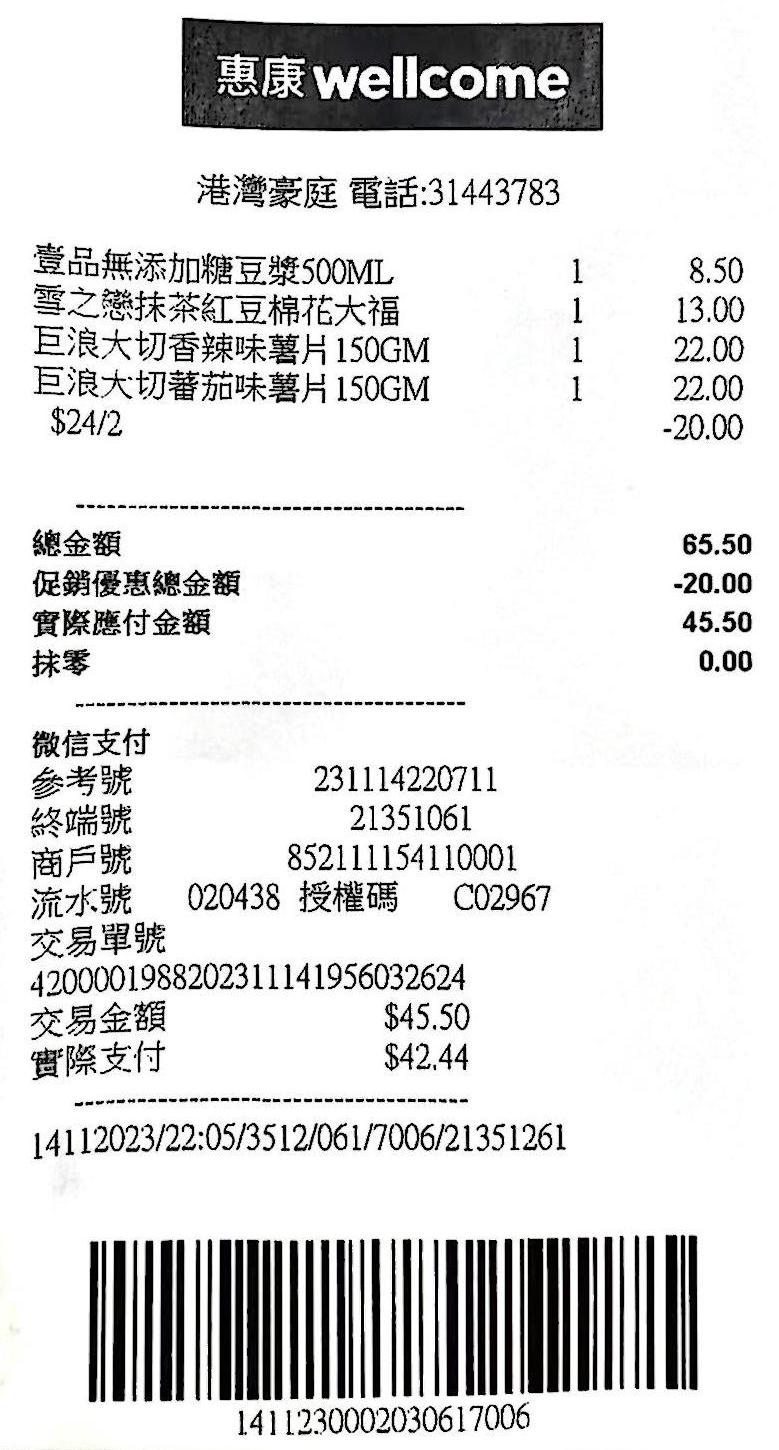
\includegraphics[width=0.45\linewidth]{image1.jpg}}
  \subcaptionbox{Wellcome Receipt 2\label{fig:receipt2}}
  {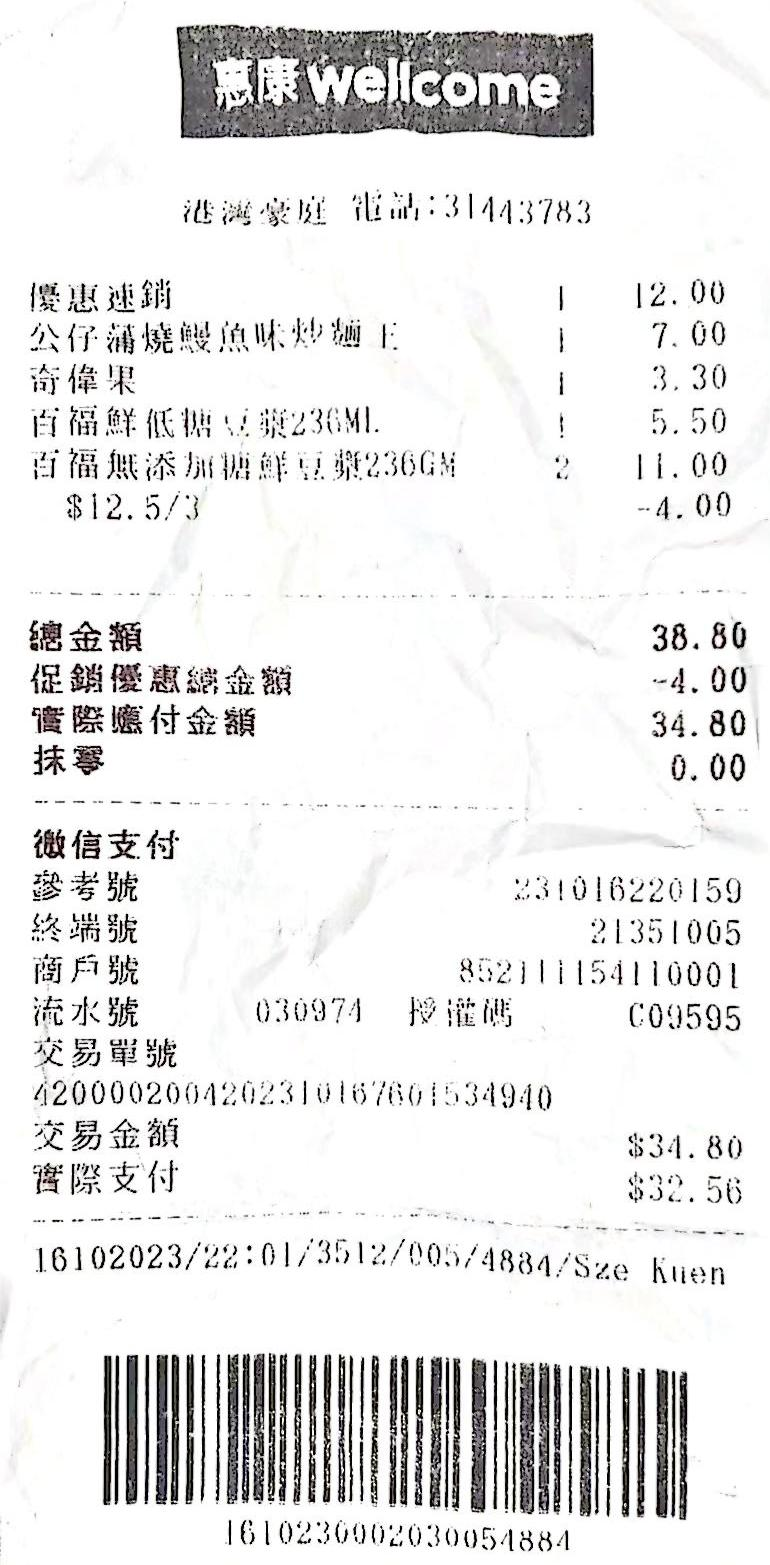
\includegraphics[width=0.45\linewidth]{image2.jpg}}
\end{figure}

\newpage



\begin{figure}
  \centering
  \subcaptionbox{HTML Display 1\label{fig:html1}}
  {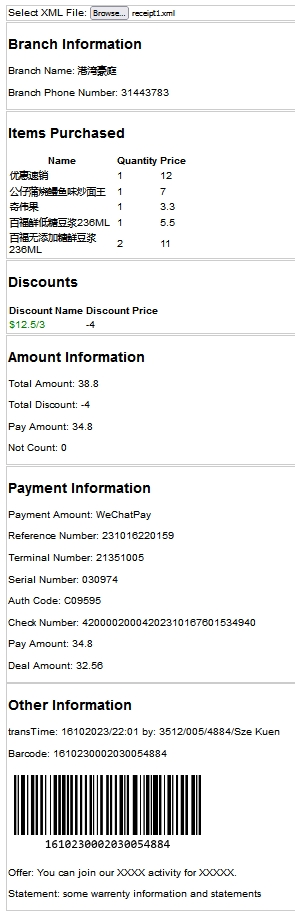
\includegraphics[width=0.45\linewidth]{html1.png}}
  \subcaptionbox{HTML Display 2\label{fig:html2}}
  {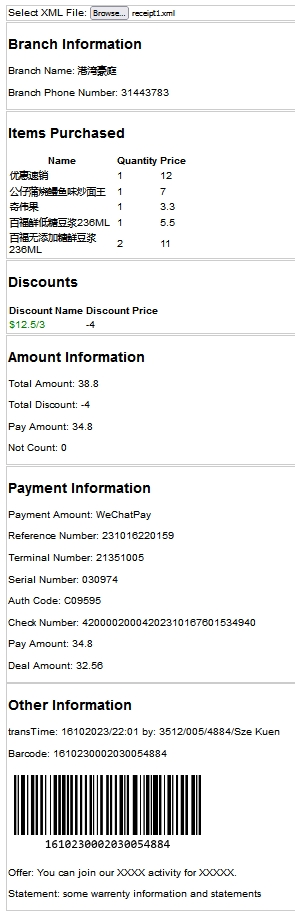
\includegraphics[width=0.45\linewidth]{html1.png}}
\end{figure}


\end{document}

